\chapter{Anhang}
\label{chap:anhang}

\section{Klassendiagramm des Tooth Analyser}
\begin{figure}[h]
	\centering
	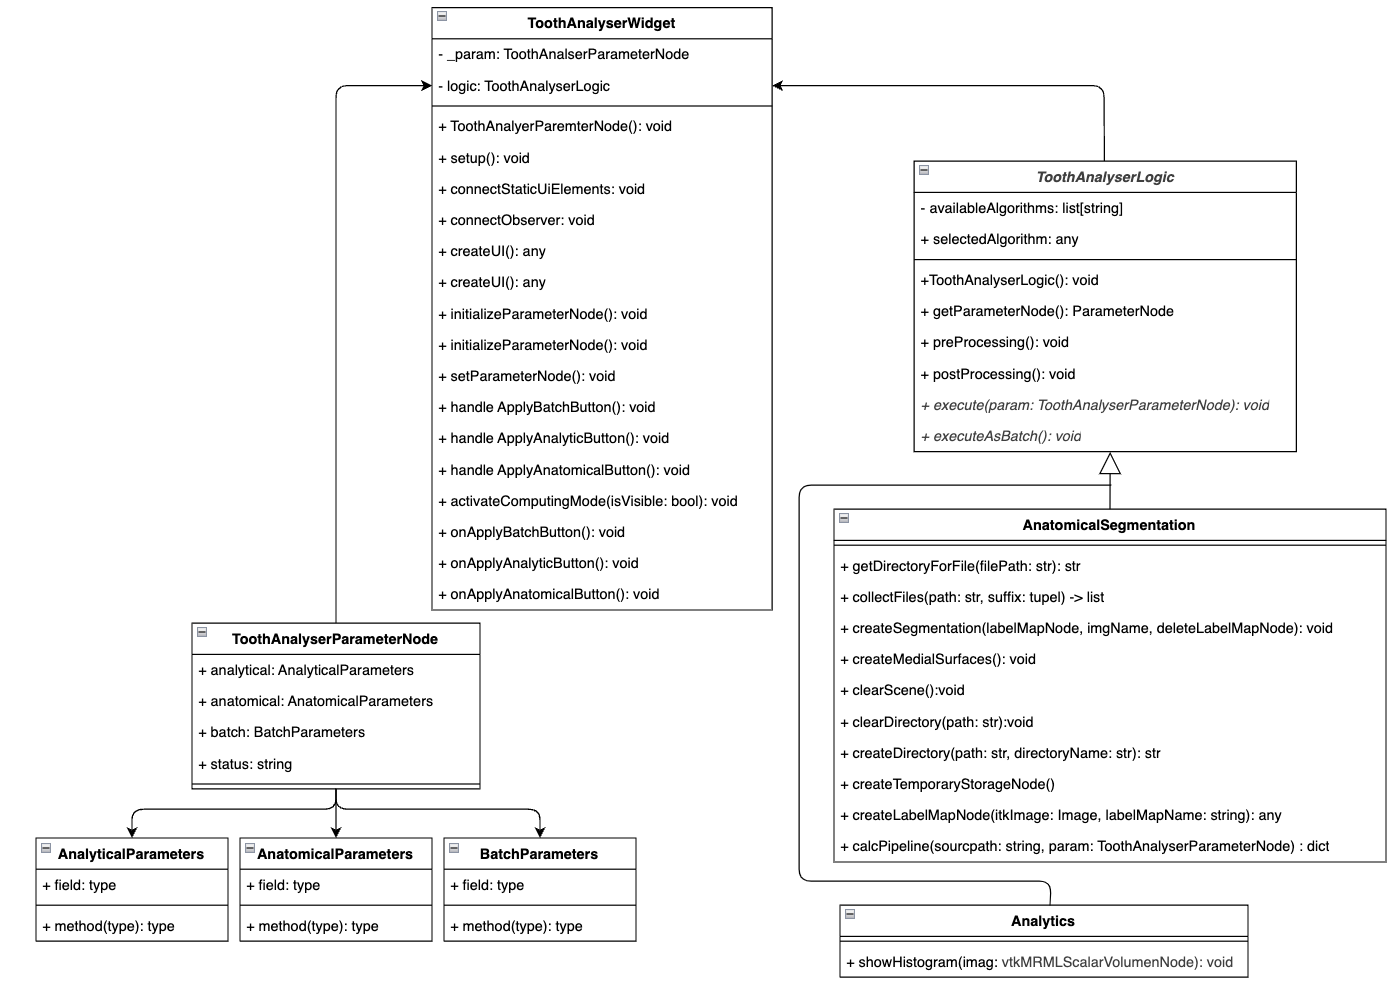
\includegraphics[width=0.9\textwidth, angle=90]{img/toothAnalyserClasses.png}
	\caption{Klassendiagramm des Tooth Analyser}
	\label{fig:klassendiagramm_gesamt}
\end{figure}
% ---------------------------------------------------------------------------------------

\section{Quellcode des Tooth Analyser}
\href{https://github.com/lukaskonietzka/SlicerToothAnalyser/blob/main/ToothAnalyser/ToothAnalyser.py}{Link
zu den Beispieldaten für die Erweiterung Tooth Analyser}
% ---------------------------------------------------------------------------------------

\section{Modul Dokumentation}
\href{https://github.com/lukaskonietzka/SlicerToothAnalyser/tree/main}{Link zur
Dokumentation für die Erweiterung Tooth Analyser}
% ---------------------------------------------------------------------------------------

\section{Beispieldaten}
\href{https://github.com/lukaskonietzka/ToothAnalyserSampleData/releases/tag/v1.0.0}{Link
zu den Beispieldaten für die Erweiterung Tooth Analyser}
% ---------------------------------------------------------------------------------------

\section{Ergebnisse des Batch-Prozesses}
Verzeichnis auf dem Galadrielrechner:\\ \texttt{/data/konietzka/Ergebnisse\_AnatomicalSegmentation\_Otsu/}
% ---------------------------------------------------------------------------------------

\section{Protokoll zur Anforderungsanalyse}
Die hier zusammengefassten Informationen stammen aus einer Besprechung und
wurden für diese Arbeit entsprechend aufbereitet. Es wird eine stichpunktartige Zusammenfassung
gefplegt.

\begin{description}
	\item[Thema:] Anforderungen für eine 3D Slicer Erweiterung ausarbeiten

	\item[Datum:] 15.07.2024

	\item[Geführt von:] Lukas Konietzka

	\item[Geführt mit:] Dr. Elias Walter 

	\item[Anwesende:] Dr. Elias Walter, Prof. Peter Rösch, Lukas Konietzka

	\item[Anforderungen:] Es existiert eine anatomische Segmentierung, liegt in
		einem IPython Notebook vor, erzielt gute Ergebnisse, soll in eine 3D Slicer
		Erweiterung eingebaut werden, anatomische Segmentierung muss von einem IPython
		Notebook irgendwie in eine Erweiterung eingebaut weden, soll eine
		Vorverarbeitung bieten, soll auch ein Batch-Prozess bieten, der Fokus soll
		erst auf die Funktion der anatomischen Segmentierung gesetzt werden, soll eventuell
		auch eine Analyse bieten.
\end{description}
% ---------------------------------------------------------------------------------------